% ------------------------------------------------------------------------
%                                Capítulo 3
% ------------------------------------------------------------------------
\chapter{Sistema de adquisición del proyecto LAGO}
% ------------------------------------------------------------------------
El proyecto LAGO esta compuesto por detectores de agua Cherenkov  ubicados en toda América latina. Estos detectores cuentan  con un sistema de adquisición electrónico que se compone de una etapa analógica para adquisición y una digital para el procesamiento de eventos relacionados con rayos cósmicos, en la Figura~\ref{sistema_adquisicion} se muestra el sistema actual, la tarjeta electrónica digitaliza pulsos de tres canales independientes a una frecuencia de 40~MHz, la FPGA es la encargada del procesamiento. La Nexys 2 y el GPS se encuentran fuera del mercado por lo cual se pone en riesgo la continuidad del proyecto. Por esta razón en este proyecto se busca actualizar la etapa de procesamiento digital haciendo uso de herramientas libres que dan independecia respecto a las FPGA en el proyecto.


En esta sección se describe la metodología usada para alcanzar cada uno de los objetivos planteados en el plan del proyecto.
Se implementa a nivel HDL los circuitos diseñados para discriminar, digitalizar y registrar aquellos pulsos que se consideran eventos.
Además se registra la hora, geolocalización del detector, temperatura y presión atmósferica. Los datos son agrupados en un archivo de salida que se entrega para su posterior análisis.

El sistema de adquisición tiene 3 canales, para lo cual se emplea el ADC AD9235 que tiene frecuencia de muestreo máxima de 50~MHz y 12 bits de resolución.
%Esta actualización del hardware de LAGO mejora la información obtenida del evento registrado.

En la Figura~\ref{sistema} se observa el sistema de adquisición de LAGO el cual se compone de los siguientes dispositivos: 

%\begin{figure}[H]
\begin{figure}[h] % Así no queda el espacio en blanco al final de la página
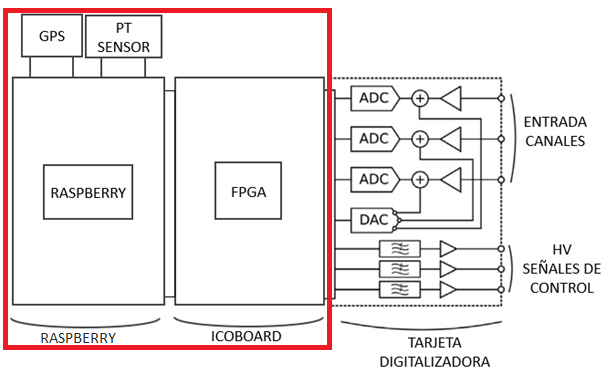
\includegraphics[scale=0.65]{Figs/pmtvie.png} 
\centering
\caption[Esquema general del sistema de adquisición actualizado]{Esquema general del sistema de adquisición actualizado, resaltando en rojo las etapas abordadas de este proyecto.} 
\label{sistema}
\end{figure}
\begin{itemize}
    \item Tarjeta electrónica que digitaliza pulsos de 3 canales independientes con salida paralela de 12 bits y una frecuencia de 50~MHz,
   \item FPGA (Icoboard) compatible con herramientas de libre desarrollo: En ella
 se implementa un conjunto de bloques jerárquicos que permiten detectar eventos relacionados con rayos cósmicos
   \item Raspberry Pi3 model B+: Permite la comunicación con los periféricos y a su vez  genera y guarda un archivo con información sobre las señales captadas y los sensores externos con el fin de establecer el tiempo de adquisición, la ubicación geográfica, la presión atmosférica y la temperatura.
   \item Dos periféricos que permitan obtener información relacionada con el entorno del WCD (ubicación, hora, temperatura ambiente y presión atmosférica.
\end{itemize}
Nota: la información proveniente de la tarjeta de digitalización será simulada con otra FPGA desde archivos existentes.\\
En la Figura~\ref{diagrama} se muestra un diagrama de bloques del sistema de adquisición implementado.
Este está compuesto por: FPGA   (Icoboard), Raspberry Pi 3   (archivo de salida), hardware externo (tarjeta de digitalización).

\begin{figure}[H]
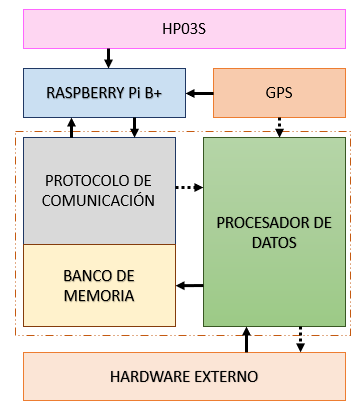
\includegraphics[scale=0.9]{Figs/hardware.PNG} 
\centering
\caption[Representación del sistema de adquisición mediante bloques]{Representación del sistema de adquisición mediante bloques. Línea discontinua: Señal de control, línea continua: Señal de control, línea discontinua naranja: FPGA.} 
\label{diagrama}
\end{figure}

%A continuación se hace una descripción funcional de cada bloque.
\section{Procesador de datos}
En la Figura~\ref{procesador} se hace una descripción funcional mediante diagrama de bloques de los circuitos de control del PMT (\texttt{RAMPA}), detección señal(\texttt{TRIGGER}), correción de línea base (\texttt{BASELINE}).

\begin{figure}[H]
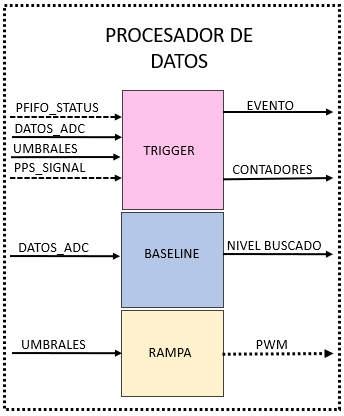
\includegraphics[scale=0.8]{Figs/procesa.PNG} 
\centering
\caption{Diagrama de bloques procesador del datos} 
\label{procesador}
\end{figure}

\subsection{Corrección de línea base}
Esta corrección se realiza con el fin de estabilizar la electrónica de adquisición frente a los efectos ambientales como la temperatura.
Es decir, si la temperatura aumenta esto provocará que la línea de base se incremente, y viceversa.
Dado que el sistema implementado compara el voltaje instantáneo en el canal ADC con una tensión de referencia (umbral de detección), cualquier cambio en el nivel de línea base podría afectar las mediciones.
Para evitar esta afectación y también el ruido electrónico se cuenta con circuitos HDL que logran mantener un valor estable de línea base en 50 niveles ADC ($\sim$49mV). 
El voltaje de línea base controlado por la FPGA se aplica a través de un convertidor de digital a analógico (DAC) de 12~bits el cual se actualiza cada 2~ms. A continuación se hace una explicación de cada uno de los bloques implementados en la FPGA para la corrección de línea base.

Para lograr una actualización de 2~ms se diseña un circuito mostrado en la Figura~\ref{actuali}  donde \textit{refresh rate} toma un valor de 100000, este valor se establece teniendo en cuenta la frecuencia del reloj de 50MHz, (período de 20 ns), entonces:
\begin{equation} \label{eq2}
     \#ciclos\times per\acute{i}odo = tiempo \rightarrow 100000 \times 20 ns = 2 ms\
\end{equation}

\begin{figure}[h]
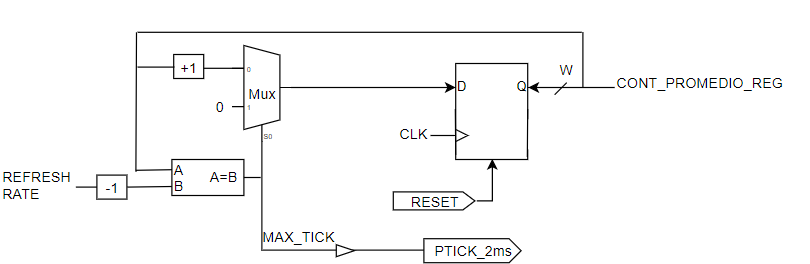
\includegraphics[width=0.9\textwidth]{Figs/CONTPROM.PNG} 
\centering
\caption{Circuito de actualización de baseline cada 2ms}
\label{actuali}
\end{figure}

El circuito de la Figura~\ref{acumulado}  muestra como los datos provenientes del ADC se acumulan durante 2~ms (MAX\_TICK) para luego hacer una comparación y lograr estabilizar la señal en $\sim$49~mV como se establece en~\citep{haro2016data}. 
El nivel de cuantización suministrado al DAC(MAX5501) se realiza en el circuito de la Figura~\ref{actu} donde se analiza la salida del acumulado (ADC\_PROM\_REG)en el contador de los ADC.

\begin{figure}[H]
\begin{minipage}[b]{0.49\linewidth}
\centering
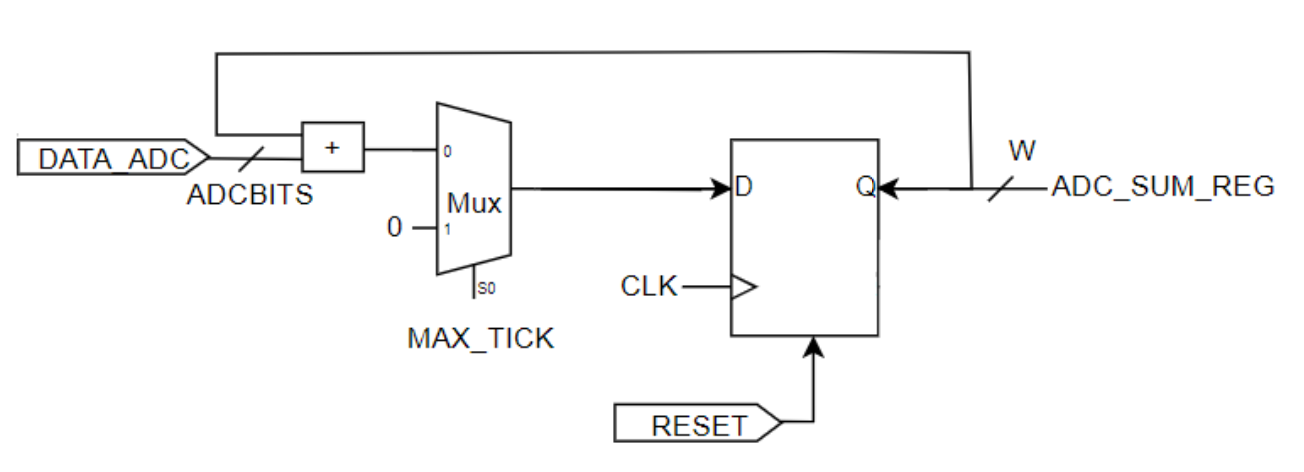
\includegraphics[width=\linewidth]{Figs/refres.PNG}
\caption{Circuito para acumular los datos provenientes de los ADC}
\label{acumulado}
\end{minipage}
\hspace{0.01cm}
\begin{minipage}[b]{0.49\linewidth}
\centering
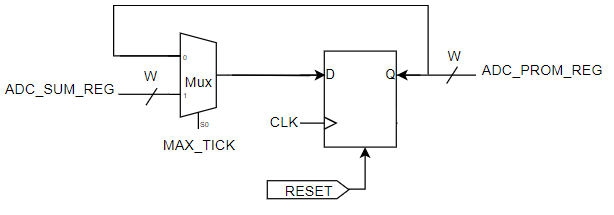
\includegraphics[width=\linewidth]{Figs/ADCPROM.PNG}
\caption{Circuito para acualizar el control de línea base cada 2~ms}
\label{actu}
\end{minipage}
\end{figure}

En ~\citep{haro2016data} se diseña un circuito inversor, cuya entrada es una señal analógica invertida. Es decir, para aumentar la salida se debe disminuir la entrada y viceversa. En el circuito Figura~\ref{salida baseline} es la señal que llega al multiplexor (MUX 2-1) y se actualiza cada 2 ms. 
Para el cálculo del módulo del circuito se tiene en cuenta los ciclos de reloj necesarios para generar 2 ms de la actualización. En este caso, el nivel de voltaje buscado coincide con 50 niveles de cuantización, como se observa en la ecuación~\eqref{eq1}
\begin{equation} \label{eq1}
    \#ciclos \times nivel\_de\_cuantizaci\acute{o}n = umbral \rightarrow 100000 \times 50 = 5000000\
\end{equation}
 
\begin{figure}[h]
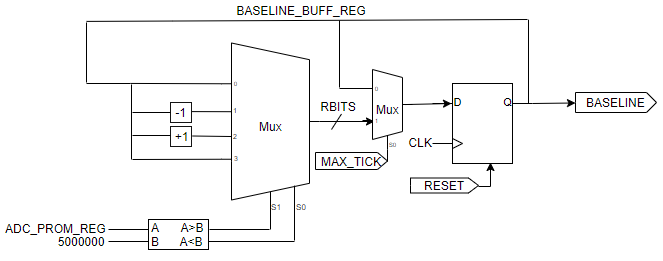
\includegraphics[scale=0.9]{Figs/base_8.PNG} 
\centering
\caption{Salida del nivel de cuantización al DAC de la línea base}
\label{salida baseline}
\end{figure}

\subsection{Regulación de  polarización de los PMT}
\label{A100}
Para el control de la fuente de alto voltaje que polariza el PMT, se genera una rampa para aumentar y/o disminuir el voltaje. 
La rampa protege los PMT de cambios bruscos de voltaje que pueden dañarlo. El usuario puede programar un set point de tensión (DATA\_IN) en el rango de 0 a 1023 en la terminal, lo que se traduce a un voltaje de 0 a 2000 V en el circuito de regulación de la fuente de polarización, como lo muestra el circuito de la Figura~\ref{registro}.

\begin{figure}[H]
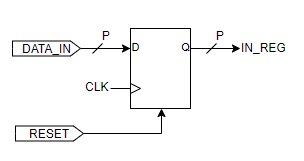
\includegraphics[scale=1]{Figs/rampa3.PNG} 
\centering
\caption{Circuito para el registro del umbral}
\label{registro}
\end{figure}

\begin{figure}[H]
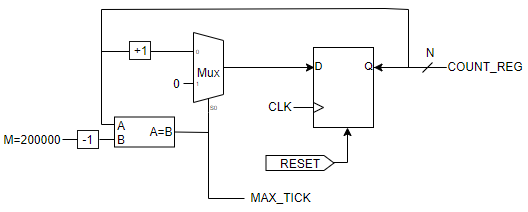
\includegraphics[scale=1]{Figs/rampa4.PNG} 
\centering
\caption{Circuito para modificar el ciclo útil de la PWM cada 2ms.}
\label{cicloutil}
\end{figure}

\begin{figure}[H]
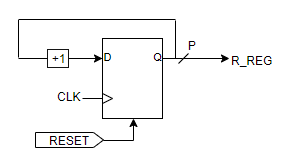
\includegraphics[scale=1]{Figs/RAMPA1.PNG} 
\centering
\caption{Circuito para generar la frecuencia de la PWM de (10~KHz)}
\label{frecuencia}
\end{figure}

El control de la PWM se establece con una frecuencia de 10~KHz se muestra en la Figura\ref{frecuencia} y una actualización cada 2ms Figura\ref{cicloutil} para lograr el control de su ciclo útil mediante la comparación respecto al umbral establecido por el usuario Figura~\ref{pwm}.
\begin{figure}[h]
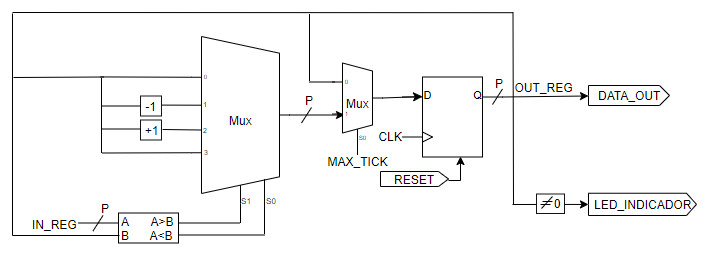
\includegraphics[width=0.9\textwidth]{Figs/RAMPA33.PNG} 
\centering
\caption[Circuito de control del ciclo útil de la PWM]{Circuito de control del ciclo útil de la PWM. (IN\_REG) es el umbral establecido por el usuario, (MAX\_TICK) actualización cada 2 ms, (OUT\_REG) es el porcentaje de ciclo útil}
\label{pwm}
\end{figure}

En el circuito de la Figura~\ref{salida} se calcula la PWM a partir de los parámetros generados anteriorimente.
(OUT\_REG) establece el porcentaje del ciclo útil y (R\_REG) la frecuencia.
De esta manera se ajusta el voltaje del PMT por medio de un conversor que interpreta la señal PWM y genera un voltaje de salida en el rango 0 a 2000V.

\begin{figure}[h]
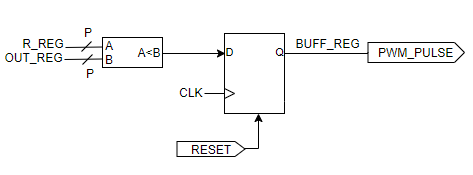
\includegraphics[scale=1]{Figs/RAMPA22.PNG} 
\centering
\caption[Circuito señal de control PWM]{, (OUT\_REG) ciclo útil, (R\_REG) frecuencia}
\label{salida}
\end{figure}


\subsection{Discriminación de datos (TRIGGER)}

La discriminación de los datos determina que pulsos son los que deben almacenarse. La condición Vi\textgreater Vthr determina que señal se considera un evento, donde Vi es la señal de entrada (DATA\_ADC) y Vthr es es el umbral (TRIGG\_SET). Según los análisis hechos .~\citep{haro2016data} un pulso completo se puede adquirir en una ventana de tiempo de 300 ns, garantizando que no se pierda información del evento adquirido. En este proyecto, son 15 muestras teniendo en cuenta la frecuencia de muestreo de 50~MHz.Todos los pulsos adquiridos se catalogan así: el conteo de pulsos registrados, el tiempo de ocurrencia y una etiqueta de 3 bits que identifica cual de los canales cumplió la condición de disparo.

La Figura~\ref{maquina} muestra una máquina de estados que controla todo el sistema de activación, esta permite controlar la información que se debe almacenar en orden secuencial en cada evento.

\begin{figure}[h!]
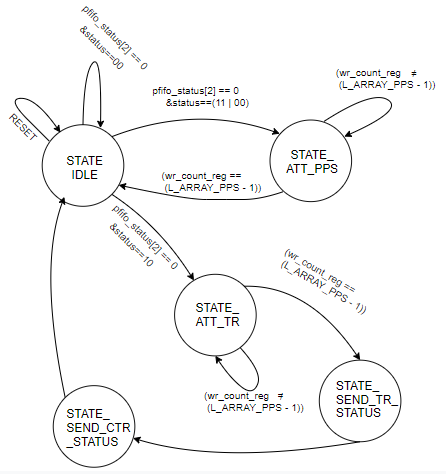
\includegraphics[width=0.8\textwidth]{Figs/fsms.PNG} 
\centering
\caption[Máquina de estados del subsistema de activación]{Máquina de estados del subsistema de activación, (STATE\_IDLE) espera, (STATE\_ATT\_PPS) reinicio de contadores cada segundo, (STATE\_ATT\_PPS) muestraeo del evento, (STATE\_SEND\_TR\_STATUS) contador del tiempo de ocurrencia del evento, (STATE\_SEND\_CTR\_STATUS) contador de eventos}
\label{maquina}
\end{figure}

El registro de desplazamiento Figura~\ref{desplazamiento} se encarga de entregar los datos provenientes de los ADC. En el registro [15] se ingresa el dato y se desplaza hasta el registro [0], esto permite hacer una comparación con el umbral de activación y  almacenar de manera simultánea la información de los 15 registros de cada canal


\begin{figure}[H]
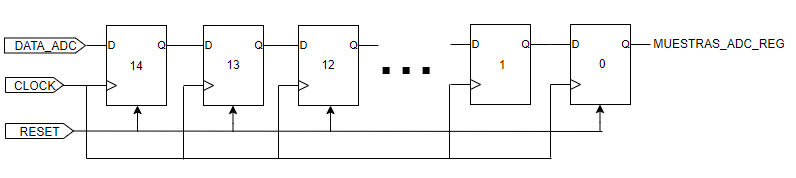
\includegraphics[width=0.9\textwidth]{Figs/registro.PNG} 
\centering
\caption{Circuito para el registro de los datos provenientes del ADC}
\label{desplazamiento}
\end{figure}

En la Figura~\ref{detectorumbral} se tiene un conjunto de comparadores conectados al registro [3, 2, 1] que determinan si el registro [3] es mayor y los registros [2,1] son menores al umbral de activación se procede a almacenar todas las posiciones del registro anterior de la siguiente manera: se concatena la información almacenada en los registros de los 3 canales y se envía la trama resultante por comunicacion SPI de modo que pasados 15 ciclos de reloj se ha comunicado todas las muestras del evento. Ver Figura~\ref{detectorumbral}
\begin{figure}[H]
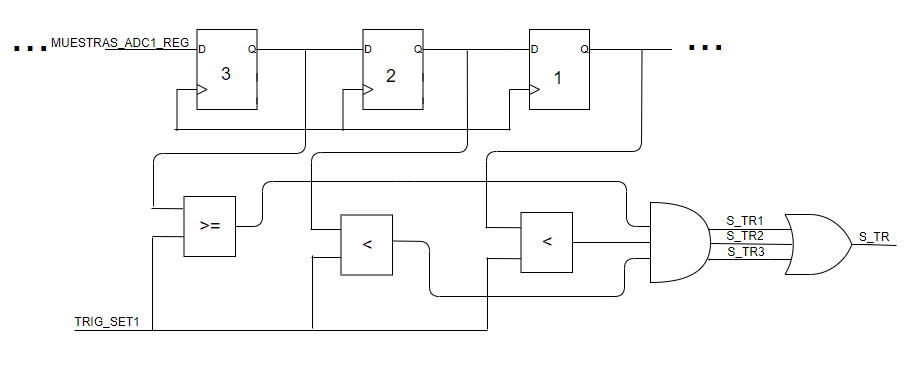
\includegraphics[width=0.9\textwidth]{Figs/COMPARA.PNG} 
\centering
\caption[Circuito de umbral de activación]{se compara la señal de entrada digitalizada(MUESTRAS$\_$ADC$\_$REG) con el umbral de activación establecido por el usuario(TRIGG$\_$SET),  si se cumple la condición de disparo se activa la señal (S$\_$TR)}
\label{detectorumbral}
\end{figure}

El circuito de la Figura~\ref{eve} concatena una bandera `10' con el contador de eventos\\ 
(CONT\_TRIGG\_REG) el cual registra el conteo de  los eventos cada vez que se cumple la condición de disparo en alguno de los 3~canales. 

\begin{figure}[h!]
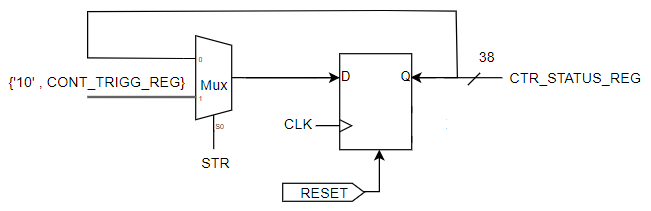
\includegraphics[scale=0.9]{Figs/ctr_status.PNG} 
\centering
\caption[Circuito concatenación trama de datos a comunicar protocolo SPI]{Circuito concatenación trama de datos a comunicar (CTR$\_$STATUS$\_$REG), (S$\_$TR) habilitador  del disparo, (CONT$\_$TRIGG$\_$REG) contador de eventos}
\label{eve}
\end{figure}

En la Figura~\ref{flancos}, el circuito se activa cada vez que se cumple la condición de disparo. Este registra el tiempo de ocurrencia, y asigna una máscara de 3 bits [S\_TR3, S\_TR2, S\_TR1] para detectar cual canal se dispara .

\begin{figure}[H]
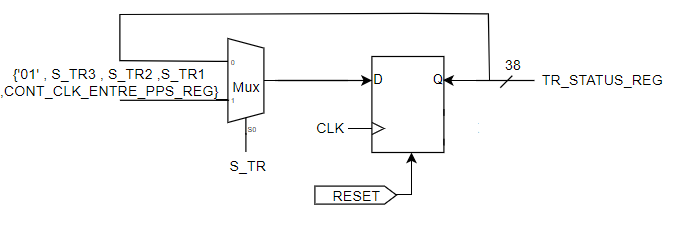
\includegraphics[scale=0.9]{Figs/tr_status.PNG} 
\centering
\caption[Circuito concatenación trama de datos a comunicar protocolo SPI ]{Circuito de concatenación de la trama de los datos a comunicar (TR$\_$STATUS$\_$REG), etiquetas de activación para cada canal (S$\_$TR3 ,S$\_$TR2, S$\_$TR1), contador tiempo entre cada evento (CONT$\_$CLK$\_$ENTRE$\_$PPS$\_$REG)}
\label{flancos}
\end{figure}

Para controlar el reinicio sincronizado de los contadores de tiempo de ocurrencia se diseña la siguiente máquina de estados que dispone de la señal pulso por segundo (PPS) la cual proviene del GPS. Ver Figura~\ref{pps}
\begin{figure}[h!]
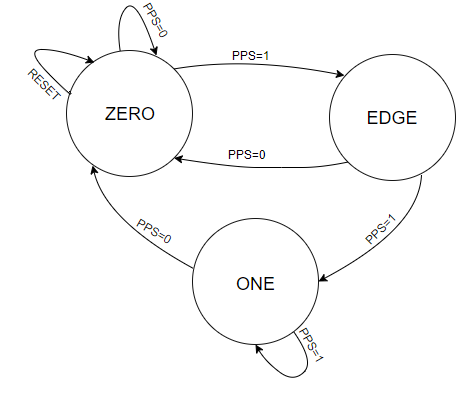
\includegraphics[scale=0.8]{Figs/MAQUINA1.PNG} 
\centering
\caption[Máquina de estados del conteo de pulsos por segundo]{Máquina de estados del conteo de pulsos por segundo, (ZERO) estado de reposo, (PPS) señal del GPS que permite activar el estado (EDGE) y por consiguiente el estado (ONE)}
\label{pps}
\end{figure}

En caso de no disponer de GPS, un circuito auxiliar divisor de frecuencia a 1 Hz se encarga de contar los flancos ascendentes del clk de la FPGA para simular la señal PPS y generar un PPS\_FALSO, con el fin de no afectar la adquisición de los eventos. Ver Figura~\ref{ppsfalso} 

\begin{figure}[H]
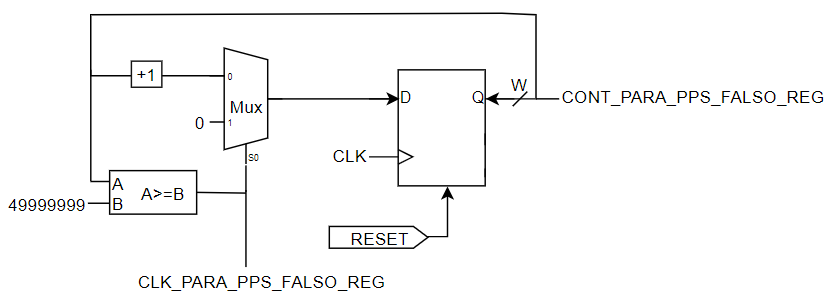
\includegraphics[width=0.9\textwidth]{Figs/CONPPSFALSO.PNG} 
\centering
\caption{Circuito de generación del PPS$\_$FALSO}
\label{ppsfalso}
\end{figure}

El circuito de la Figura~\ref{comparafalso} modula el ciclo útil del PPS\_FALSO a 100 ms.

\begin{figure}[H]
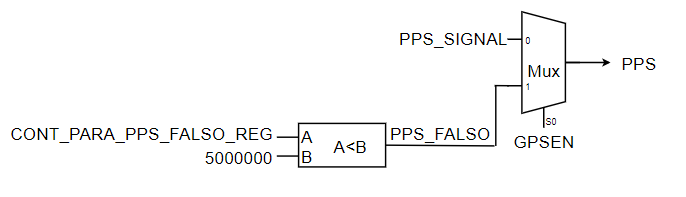
\includegraphics[scale=0.8]{Figs/PPSP.PNG} 
\centering
\caption[Circuito para generar la señal PPS]{Circuito para generar la señal PPS, selecciona la señal proveniente del GPS (PPS$\_$SIGNAL) o una señal simulada (PPS$\_$FALSO), en caso de ausencia del GPS (GPSEN)}
\label{comparafalso}
\end{figure}

Si se activa el PPS\_FALSO se activa un led de indicación se muestra en la Figura~\ref{ledfalso}
\begin{figure}[H]
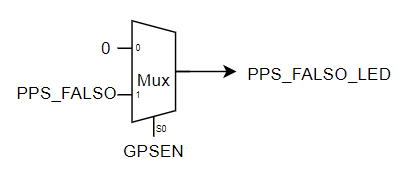
\includegraphics[scale=0.8]{Figs/TRIGER5.PNG} 
\centering
\caption{Circuito de activación de PPS\_FALSO\_LED}
\label{ledfalso}
\end{figure}

\section{\textbf{Protocolo de comunicación}}
Este bloque logra la comunicación entre la FPGA y la Raspberry para la transmisión y recepción de la información; el protocolo se basa en el estándar SPI, donde la Raspberry es el maestro y la FPGA el esclavo. Este protocolo fue elegido teniendo en cuenta que la tasa de detección de un WCD típico en LAGO puede alcanzar valores hasta de 2 KHz.~\citep{hernandez2018procedimiento}

\begin{figure}[H]
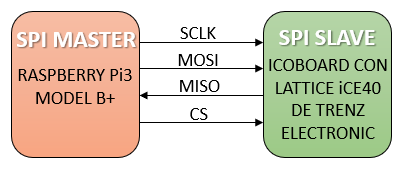
\includegraphics[scale=1]{Figs/SPIPROTO.PNG} 
\centering
\caption[Esquema protocolo SPI]{Protocolo SPI se compone de 4 señales así: SCLK señal de reloj proviniente del maestro Raspberry Pi 3, MOSI señal que permite llevar los bits del maestro hacia el esclavo, MISO señal que permite llevar los bits del esclavo al maestro y CS señal que se encarga de habilitar el esclavo} 
\label{adecuacion}
\end{figure}

El protocolo SPI utilizado en el proyecto fue basado en .~\citep{charkster/spi_slave_verilog_2020} en el cual se implementa un  SPI Slave y un mapa de memoria diseñado para la comunicación entre una FPGA y una Raspberry. En la Figura~\ref{spi} se muestra el RTL(Register-transfer-level) del protocolo implementado.

\begin{figure}[H]
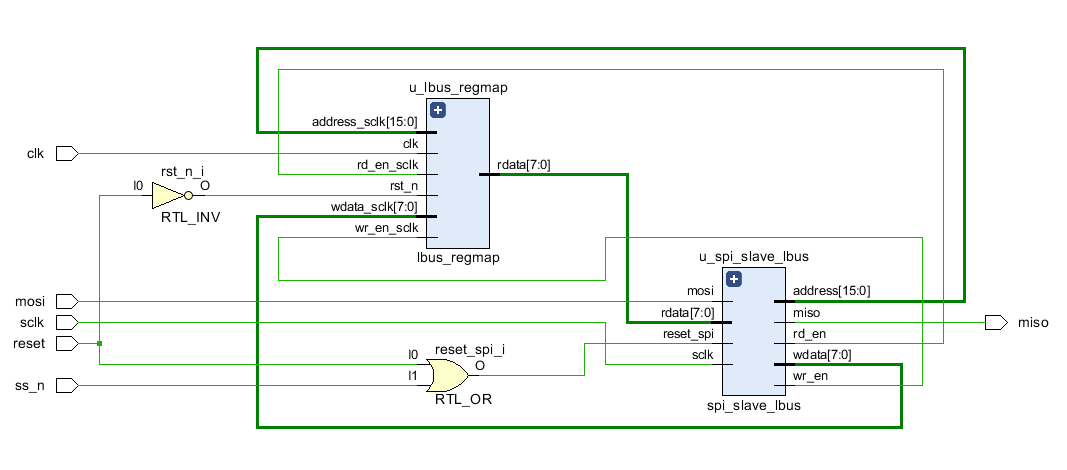
\includegraphics[width=0.93\textwidth]{Figs/rtlproto.PNG} 
\centering
\caption{RTL protocolo de comunicación SPI .~\citep{XilinxInc.2016IntegratedGuide}} 
\label{spi}
\end{figure}

El mapa de memoria del protocolo se modifica y redimensiona para almacenar los eventos provenientes de los ADC.
La Tabla~\ref{tab:my-table} muestra como se ha distribuido los datos transferidos y la posición de memoria asignada para cada uno, obteniendo una totalidad de 98 posiciones con un ancho de 8 bits para cada una.

\begin{table}[h!]
\centering
\begin{tabular}{|c|c|c|c|c|}
%\hline
%\multicolumn{5}{|c|}{\cellcolor[HTML]{E0E0E0} MAPA DE MEMORIA PROTOCOLO SPI }\\
\hline
%\multicolumn{2}{|c|}{Posición} &  & \multicolumn{1}{l|}{}&\\
Posición & Posición      & & Bits & \\ 
Inicial & Final         & \multirow{-2}{*}{Dato} & usados & \multirow{-2}{*}{Descripción}\\
\hline
 0 &  1 & Trigger 1     & 12 & \\ \cline{1-4}
 2 &  3 & Trigger 2     & 12 & \\ \cline{1-4}
 4 &  5 & Trigger 3     & 12 & \\ \cline{1-4}
 6 &  7 & Rampa 1       & 12 & \\ \cline{1-4}
 8 &  9 & Rampa 2       & 12 & \\ \cline{1-4}
10 & 11 & Rampa 3       & 12 & \multirow{-6}{*}{\begin{tabular}[c]{@{}c@{}}Parámetros\\
                                ingresados\\ por usuario\end{tabular}} \\ \hline
12 & 12 & Pfifo\_status & 1  & Señal de control \\ \hline
13 & 17 & Muestra 1     & 38 & \\ \cline{1-4}
18 & 22 & Muestra 2     & 38 & \\ \cline{1-4}
23 & 27 & Muestra 3     & 38 & \\ \cline{1-4}
28 & 32 & Muestra 4     & 38 & \\ \cline{1-4}
33 & 37 & Muestra 5     & 38 & \\ \cline{1-4}
38 & 42 & Muestra 6     & 38 & \\ \cline{1-4}
43 & 47 & Muestra 7     & 38 & \\ \cline{1-4}
48 & 52 & Muestra 8     & 38 & \\ \cline{1-4}
53 & 57 & Muestra 9     & 38 & \\ \cline{1-4}
58 & 62 & Muestra 10    & 38 & \\ \cline{1-4}
63 & 67 & Muestra 11    & 38 & \\ \cline{1-4}
68 & 72 & Muestra 12    & 38 & \\ \cline{1-4}
73 & 77 & Muestra 13    & 38 & \\ \cline{1-4}
78 & 82 & Muestra 14    & 38 & \\ \cline{1-4}
83 & 87 & Muestra 15    & 38 & \\ \cline{1-4}
88 & 92 & Contador 1    & 38 & \\ \cline{1-4}
93 & 97 & Contador 2    & 38 & \multirow{-17}{*}{\begin{tabular}[c]{@{}c@{}}Trama\\ de datos\\ evento\end{tabular}}  \\
\hline
\end{tabular}
\caption{Mapa de memoria protocolo SPI}
\label{tab:my-table}
\end{table}

%\newpage
\section{\textbf{Hardware externo de emulación}}

Teniendo en cuenta que este proyecto se compone sólo de la parte digital del sistema DAQ de LAGO. Los datos de eventos que pueden ser considerados rayos cósmicos fueron simulados desde un archivo de salida ya existente. Estos fueron almacenados en las memorias ROOM de una FPGA Nexys 4-DDR (nombrada de ahora en adelante solo Hardware externo) para simular el ADC en condiciones de detección.
Con esta estrategia se consigue simular la electrónica de digitalización.

El Hardware externo recibe una señal de reloj a 50MHz proveniente de la FPGA Icoboard para sincronizar la de información almacenada en las memorias. 
 
\begin{figure}[h]
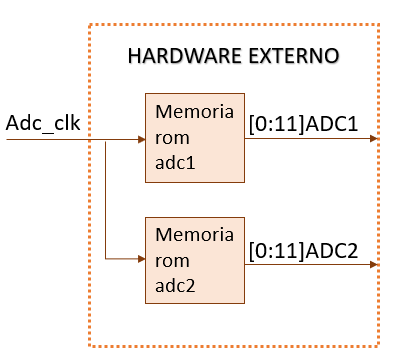
\includegraphics[scale=0.7]{Figs/hardexter.PNG} 
\centering
\caption[Diagrama de bloques hardware externo]{Diagrama de bloques hardware externo, Adc\_clk es la señal de reloj transmitida por la Icoboard}
\label{adecuacion}
\end{figure}
Ha sido necesario incluir una descripción  que permite sincronizar en frecuencia y fase los relojes de las dos FGPA y así asegurar que las muestras se entreguen sin pérdida de información por violación de tiempos.

\section{Raspberry pi 3 B+}

\begin{figure}[H]
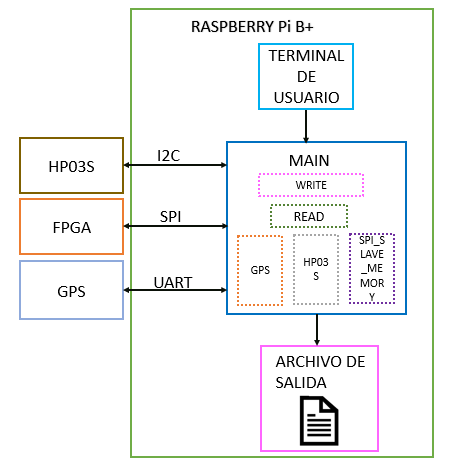
\includegraphics[scale=0.8]{Figs/raspidiagrama.PNG} 
\centering
\caption{Diagrama de bloques Raspberry Pi}
\label{rasp}
\end{figure}

La Raspberry almacena las tramas de datos que componen un evento y registra los datos obtenidos de tres dispositivos que conforman el sistema de adquisición a través de diferentes protocolos de comunicación como se muestra en la Figura~\ref{rasp}.
\begin{itemize}
    \item Protocolo SPI para la FPGA Icoboard: permitiendo acceder a los registros para configurar parámetros de adquisición y envío de los eventos registrados. 
    \item Protocolo I2C para el sensor HP03S: por medio de la librería wiringPiI2C se configura la comunicación según. ~\citep{HP03SDatasheet}.
    \item Protocolo UART con sensor GPS: se obtiene lectura hora y  geoposicionamiento según. ~\citep{Adafruit2020}.

\end{itemize}


%La comunicación con el sensor HP03S se logra con I2C según la   hoja de datos ~\citep{HP03SDatasheet},importando librerías al    software como <wiringPiI2C>.
 
%La comunicación con el GPS se realiza a través del protocolo UART para lograr la lectura y escritura de los datos de hora y geoposicionamiento al software ~\citep{Adafruit2020}.

Finalmente el archivo \texttt{Main} corresponde a un \textit{script} en Python donde se establece el llamado de todas las funciones, recopilando toda la información.
Además, se crea una interfaz de usuario para el ingreso de parámetros por medio de una terminal.
Posteriormente se entrega un archivo de salida que presenta el registro de los eventos.





%----------------------------------------------------------------------------------------------------------------